\documentclass{article}\usepackage[]{graphicx}\usepackage[]{xcolor}
% maxwidth is the original width if it is less than linewidth
% otherwise use linewidth (to make sure the graphics do not exceed the margin)
\makeatletter
\def\maxwidth{ %
  \ifdim\Gin@nat@width>\linewidth
    \linewidth
  \else
    \Gin@nat@width
  \fi
}
\makeatother

\definecolor{fgcolor}{rgb}{0.345, 0.345, 0.345}
\newcommand{\hlnum}[1]{\textcolor[rgb]{0.686,0.059,0.569}{#1}}%
\newcommand{\hlstr}[1]{\textcolor[rgb]{0.192,0.494,0.8}{#1}}%
\newcommand{\hlcom}[1]{\textcolor[rgb]{0.678,0.584,0.686}{\textit{#1}}}%
\newcommand{\hlopt}[1]{\textcolor[rgb]{0,0,0}{#1}}%
\newcommand{\hlstd}[1]{\textcolor[rgb]{0.345,0.345,0.345}{#1}}%
\newcommand{\hlkwa}[1]{\textcolor[rgb]{0.161,0.373,0.58}{\textbf{#1}}}%
\newcommand{\hlkwb}[1]{\textcolor[rgb]{0.69,0.353,0.396}{#1}}%
\newcommand{\hlkwc}[1]{\textcolor[rgb]{0.333,0.667,0.333}{#1}}%
\newcommand{\hlkwd}[1]{\textcolor[rgb]{0.737,0.353,0.396}{\textbf{#1}}}%
\let\hlipl\hlkwb

\usepackage{framed}
\makeatletter
\newenvironment{kframe}{%
 \def\at@end@of@kframe{}%
 \ifinner\ifhmode%
  \def\at@end@of@kframe{\end{minipage}}%
  \begin{minipage}{\columnwidth}%
 \fi\fi%
 \def\FrameCommand##1{\hskip\@totalleftmargin \hskip-\fboxsep
 \colorbox{shadecolor}{##1}\hskip-\fboxsep
     % There is no \\@totalrightmargin, so:
     \hskip-\linewidth \hskip-\@totalleftmargin \hskip\columnwidth}%
 \MakeFramed {\advance\hsize-\width
   \@totalleftmargin\z@ \linewidth\hsize
   \@setminipage}}%
 {\par\unskip\endMakeFramed%
 \at@end@of@kframe}
\makeatother

\definecolor{shadecolor}{rgb}{.97, .97, .97}
\definecolor{messagecolor}{rgb}{0, 0, 0}
\definecolor{warningcolor}{rgb}{1, 0, 1}
\definecolor{errorcolor}{rgb}{1, 0, 0}
\newenvironment{knitrout}{}{} % an empty environment to be redefined in TeX

\usepackage{alltt}

\usepackage[letterpaper,top=2cm,bottom=2cm,left=3cm,right=3cm,marginparwidth=1.75cm]{geometry}

\usepackage{amsmath, amsfonts, amssymb, mathtools}
\usepackage{accents}
\usepackage{graphicx}
\usepackage{algorithm}
\usepackage[noend]{algpseudocode}
\usepackage{amsthm}
\usepackage{bm}
\usepackage{cases}
\usepackage{caption}
\usepackage{soul}
\usepackage{tikz}
\usepackage{pgfplots}
\usepackage{float}
\usepackage{xr-hyper}
\usepackage{hyperref}
\externaldocument{alloscore-application}

\usepackage{enumitem}
\newlist{todolist}{itemize}{2}
\setlist[todolist]{label=$\square$}
\usepackage{pifont}
\newcommand{\cmark}{\ding{51}}%
\newcommand{\xmark}{\ding{55}}%
\newcommand{\done}{\rlap{$\square$}{\raisebox{2pt}{\large\hspace{1pt}\cmark}}%
\hspace{-2.5pt}}
\newcommand{\wontfix}{\rlap{$\square$}{\large\hspace{1pt}\xmark}}

\DeclareMathOperator*{\argmin}{argmin}
\DeclareMathOperator{\short}{sh}
\DeclareMathOperator{\Ex}{\mathbb{E}}


\usepackage{setspace}


\usepackage{parskip}

\usepackage{soul}
\usepackage{xcolor}
\def\elr#1{{\color{cyan}\textbf{ELR:[#1]}}}
\def\apg#1{{\color{red}\textbf{APG:[#1]}}}
\def\bwr#1{{\color{violet}\textbf{BWR:[#1]}}}
\def\ngr#1{{\color{blue}\textbf{NGR:[#1]}}}

\usepackage{natbib}
\bibliographystyle{unsrtnat}

\title{Supplementary Material for ``Evaluating infectious disease forecasts with allocation scoring rules''}
\author{Aaron Gerding, Nicholas G. Reich, Benjamin Rogers, Evan L. Ray}
\IfFileExists{upquote.sty}{\usepackage{upquote}}{}
\begin{document}

\newcommand{\del}[2]{\frac{\partial {#1} }{\partial {#2}} }
\newcommand{\dby}[2]{\frac{d {#1} }{d {#2}} }
\newcommand{\sbar}{\overline{s}}

\newtheorem{proposition}{Proposition}

\theoremstyle{remark}
\newtheorem*{remark}{Remark}

\maketitle







\begin{abstract}
We briefly address some technical and methodological points in the main text, referring to the forthcoming ... for 
more thorough discussion.
\end{abstract}

\begin{todolist}
	\item[\done] From 2.2.1, why are Bayes act scoring rules proper?
	%\item Explain ``All proper scoring rules for probabilistic forecasts have an explicit link to a loss function'' from discussion.
	\item DGP as optimal for any decision problem, ref Diebold, Gunther, Tay p. 866; and if forecasts are ideal, then forecasts with better information always yield better decisions, ref Holzmann and Eulert, Corr 2.
	\item[\done] For 2.2.2, how to get quantile representation of Bayes act using Lagrange multiplier, \st{assuming smooth, never-zero densities well behaved at $x=0$.} Work out exponential example. Refer to methods paper for general case.
	\item[\done] Derivation of quantile scoring rule with quantile as Bayes act for C/L problem, \st{assuming never-zero densities}. 
	\item algorithmic details
	\begin{todolist}
		\item use of \texttt{distfromq} to get from quantiles to distribution functions
		\item \texttt{alloscore}
		\item implications for propriety. do quantiles elicited by \texttt{distfromq} $\hookrightarrow$ \texttt{alloscore} process align with ``real'' quantiles? the alloscore is proper if distribution functions F are handed to us; is it still proper given our algorithm situation?
	\end{todolist}

	\item Descriptions of 
		\begin{todolist}		
			\item CRPS as average quantile score across $C \in [0/L]$ decision problems
			\item IS as average of two quantile scores with a prob-width penalty
			\item WIS as average quantile score across 23 C/L problems.
		\end{todolist}
	%item Sketch of scoring for decision problems involving both cost and constraint.
	\item[\xmark]  Derivation of case 2 in formula for Oracle adjustment (done in manuscript?)
\end{todolist}

\section{Introduction}
\label{sec:intro}

We briefly address some technical and methodological points in the main text. We begin in section \ref{sec:shortage} by formalizing the concept of a \emph{shortage} of resources and giving some key results about expected resource shortages under a distribution characterizing uncertainty about (future) levels of resource need. Resource shortages play a central role in the decision-making problems that give rise to the quantile loss and the allocation score, which we discuss in sections \ref{sec:quantiles_shortage} and \ref{sec:bayes-quantiles} respectively. Section \ref{sec:numeric} gives details on the numerical methods that we use to calculate allocation scores, including some special considerations for settings where forecasts are represented by a finite collection of predictive quantiles, such as the application to forecasts of hospitalizations due to COVID-19 in section 3 of the article.

\section{Shortages}
\label{sec:shortage}

We use $y$ to denote the demand or need for resources and $x$ to denote the level of available resources.
The resource shortage is the amount by which resource demand exceeds supply. 
For convenience, we write $u_{+} = \max\{0,u\}$, i.e., ``the positive part'' of $u$.
With this notation, the shortage is written as $(y - x)_{+}$. To regard shortage as a function of only one 
variable $x$ or $y$, with the other being a parameter describing the dependence we can write 
$(y - x)_{+} = \short^{y}(x) = \short_{x}(y)$.  Note that 
$\short^{y}(x)$ and $\short_{x}(y)$ are both convex functions and ``mirror'' each other (see figure \ref{fig:shortages}).

\pgfplotsset{compat=1.16} % Set the compatibility of pgfplots
\begin{figure}[H]
\begin{tikzpicture}
\begin{axis}[
    axis lines=middle, % Center the axis
    xmin=0, xmax=10, % Set the range for the x-axis
    ymin=0, ymax=10, % Set the range for the y-axis
    xlabel={$x$ or $y$},
    ylabel={shortage},
    xtick={4, 6}, % Set the position of the ticks on the x-axis
    ytick=\empty, % No ticks on the y-axis
    xticklabels={$x_0$, $y_0$}, % Label for the tick on the x-axis
    clip=false,
    every axis x label/.style={at={(current axis.right of origin)},anchor=north west},
    every axis y label/.style={at={(current axis.above origin)},anchor=south east}
]

% Add the plot for max(0, y_0 - x)
\addplot+[sharp plot, no marks, thick, blue] coordinates {(0,6) (6,0) (10,0)}
node[pos=.1,anchor=south west] {$\short^{y_0}(x) = (y_0 - x)_{+}$}; % Label for the first function


% Add the plot for max(0, y - x_0)
\addplot+[sharp plot, no marks, thick, red, ->] coordinates {(0,0) (4,0) (10,6)}
node[pos=.7,anchor=north west] {$\short_{x_0}(y) = (y - x_0)_{+}$};

\end{axis}
\end{tikzpicture}
\caption{Shortage functions. $\mathrm{sh}^{y_0}(x)$, shown in blue, gives the resource shortage as a function of the level of available resources, $x$, for a fixed value of resource demand $y_0$. $\mathrm{sh}_{x_0}(y)$, shown in red, gives the resource shortage as a function of resource demand, $y$, for a fixed value of resource supply $x_0$.}
\label{fig:shortages}
\end{figure}

Let $Y$ be a random variable with distribution $F$ representing the unknown level of resource demand. The random shortage $(Y-x)_{+}$ can be thought of as either a 
real-valued random variable $\short_x(Y)$ for every $x$, or a function-valued random variable $\short^Y$ whose value
for any realization $Y=y$ is a convex function $\short^y(x)$ of $x$.  In the sections below, we will work with the 
\emph{expected shortage}\footnote{A more natural sounding term for $(y-x)_{+}$ might have been \emph{shortfall}. Unfortunately 
\emph{expected shortfall} has long been used in finance to refer to quantities more 
closely related to the \emph{conditional} expectation $\Ex_F [Y-x \mid Y - x \geq 0] = \Ex_F [(Y-x)_{+}]/\mathbb{P}_F\{Y \geq x\}$.}
$\Ex_F [(Y-x)_{+}] = \Ex_F[\short^Y](x)$.
Assuming that this expected value exists, which is the case as long as the distribution $F$ is well behaved, we can see that $\Ex_F[\short^Y](x)$ is also convex (and therefore continuous) in $x$ by integrating the convexity inequality for
$\short^y(x)$ with respect to the probability measure $dF(y)$:
\begin{align}
	\Ex_F[\short^Y](\lambda x_1+(1-\lambda) x_2) &= \int \short^y(\lambda x_1+(1-\lambda) x_2)dF(y) \nonumber \\
	&\leq \int \lambda\short^y(x_1) +(1-\lambda) \short^y(x_2)dF(y) \nonumber \\
	&=\lambda\Ex_F[\short^Y](x_1) + (1-\lambda)\Ex_F[\short^Y](x_2). \label{eqn:convex-esf}
\end{align}
Convexity is also shown by directly exhibiting the the left and right derivatives of $\Ex_F[\short^Y](x)$:
\begin{align}
D_{-}\Ex_F [(Y-x)_{+}] &= \lim_{h \searrow 0}\frac{1}{h}\Ex_F [(Y - x)_{+} - (Y - (x - h))_{+}] \\
&= \lim_{h \searrow 0}\frac{1}{h}\int_{[x\mathrlap{-h, x]}} (x - h - y) dF(y) - 
\lim_{h \searrow 0}\frac{1}{h}\int_{(x\mathrlap{,\infty)}} h dF(y)  \\
&= \lim_{h \searrow 0}\frac{1}{h}\int_{[x\mathrlap{-h, x]}} - h dF(y) - 1 + F(x) \label{eqn:dsfllim} \\
&= -(F(x) - F(x-)) - 1 + F(x) \quad \left(\text{where } F(x-) := \lim_{t \nearrow x} F(t)\right)\\
&= F(x-) - 1  \label{eqn:dsfl} \\
D_{+}\Ex_F [(Y-x)_{+}] &= \lim_{h \searrow 0}\frac{1}{h}\Ex_F [(Y - (x + h))_{+} - (Y - x)_{+}] \\
&= \lim_{h \searrow 0}\frac{1}{h}\int_{[x\mathrlap{, x+h]}} (x - y) dF(y) - 
\lim_{h \searrow 0}\frac{1}{h}\int_{(x\mathrlap{+h,\infty)}} h dF(y)  \\
&= \lim_{h \searrow 0}\frac{1}{h}\int_{[x\mathrlap{, x+h]}} 0 dF(y) - 1 + F(x) \label{eqn:dsfrlim} \\
&= F(x) - 1 \label{eqn:dsfr}
\end{align}
where in \eqref{eqn:dsfllim} and \eqref{eqn:dsfrlim} we are able to replace the integrands with their values at $x$ because 
they are bounded over the shrinking regions of integration $[x-h,x]$ and $[x,x+h]$. Convexity follows since 
$D_{-}\Ex_F[\short^Y](x) \leq D_{+}\Ex_F[\short^Y](x)$ by the definition of $F(x)$ and $F(x-)$. This also shows that if $F$ does not 
have a point mass at $x$, we have 
\begin{align}
	\frac{d}{dx} \Ex_F [(Y-x)_{+}] = F(x)-1,
\end{align}
coinciding with the ``Leibniz rule'' calculation
\begin{align}
	\frac{d}{dx} \Ex_F [(Y-x)_{+}] &= \frac{d}{dx} \int_{x}^{\infty} (y-x) f_Y(y)dy \\
	&= \int_{x}^{\infty} \frac{d}{dx}(y-x) f_Y(y)dy - (x-x) f_Y(x) = -\int_{x}^{\infty} f_Y(y)dy = F(x)-1.
\end{align}
which assumes $Y$ has an adequately well-behaved density $f_Y$.


\section{Quantiles and Expected Shortage}
\label{sec:quantiles_shortage}

We recall how quantiles arise as solutions to a probabilistic decision problem, drawing on perspectives developed in the fields of
both forecasting (see e.g., \cite{gneiting2011quantiles} and \cite{jose2009evaluating}) and stochastic optimization 
(se e.g., \cite{royset2022optimization}, sections 1.C and 3.C).

Let $Y$ be a random variable
representing the future level of an undesirable outcome such as severe COVID incidence. Let $x \in \mathbb{R}_+$ be a decision variable
representing levels of some costly counter-measure, such as procurement of monoclonal antibody treatments,
that can be taken at a cost $C>0$ per unit in preparation for $Y$.\footnote{
Quantiles could also be derived for a problem in which $x$ and $Y$ take negative values, corresponding, for instance, to a decision
maker that both buys and sells in a resource market and a $Y$ that takes negative values when ``recoveries'' outnumber incidence.  
But we do not consider such scenarios in this work.	 
}  A decision maker must decide on a level $x$ of investment in the
counter-measure, and wishes to avoid excesses in either the expediture $Cx$ or the shortage $(y-x)_{+}$ when $Y=y$ is
realized. To formalize the trade-off between these potential excesses we quantify the loss associated with a unit of
shortage by a constant $L>C$ (which assumes that the counter-measure has some practical value) and combine the total shortage loss with expenditure into a \emph{loss function}\footnote
{This does involve a confusing use of the word \emph{loss} to refer to two different quantities, but this seems to be
an ingrained and unavoidable habit in the literature.}
\[
l(x,y) = Cx + L(y-x)_{+}.
\] 
The decision problem is then to select an action $x$ that aligns with the preference that $l(x,y)$ be
as low as possible given any realization $Y=y$.  Equivalently, the problem is to choose a random future loss $l(x,Y)$ which
is \emph{admissible}, meaning that there is no alternative action $\tilde{x}$ producing a random future loss $l(\tilde{x},Y)$
which is never greater than $l(x,Y)$ and strictly lower for some realization $Y=y_0$.

Admissibility with respect to the loss $l$ is not, however, by itself a very strong decision criterion.
To give the decision problem more structure we assume the decision maker either knows the distribution $F$ of $Y$, or
wishes to proceed as if a forecast $F$ of $Y$ were true. This gives us what is known in decision theory as a decision
problem \emph{under risk} (regarding the future value of $Y$) as opposed to one \emph{under uncertainty} where both $Y$
as well as $F$ are unknown when the decision is to be made. A principle commonly invoked in this situation\footnote
{Note that this priciple might be inappropriate when the decision maker is \emph{risk averse} in some way such as
having a preference for random losses with lower variance.} is that the decision maker should or will seek to minimize the expected
loss
\begin{align}
  \mathbb{E}_{F}[l(x,Y)] = Cx + L\mathbb{E}_{F}[(Y-x)_{+}]. \label{eqn:expQloss}
\end{align}

The expected loss is an affine transformation of the convex expected shortage (c.f. \eqref{eqn:convex-esf}). Therefore
$\mathbb{E}_{F}[l(x,Y)]$ is also is convex and has right and left derivatives $D_{\pm}\mathbb{E}_{F}[l(x,Y)]$ at every $x$. 
Because these derivatives exist everywhere, a necessary condition for $x^{\star}$ to
minimize $\mathbb{E}_{F}[l(x,Y)]$ is that $D_{+}\mathbb{E}_{F}[l(x^{\star},Y)] \geq 0$ and 
$D_{-}\mathbb{E}_{F}[l(x^{\star},Y)] \leq 0$, and because of convexity, this condition is also sufficient. From \eqref{eqn:dsfl} 
and \eqref{eqn:dsfr} this means that
\begin{align}
D_{+}\mathbb{E}_{F}[l(x^{\star},Y)] = C + L(F(x^{\star}) - 1) \geq 0 \geq 
D_{-}\mathbb{E}_{F}[l(x^{\star},Y)] = C + L(F(x^{\star}-) - 1) \label{eqn:expQd-ineq}
\end{align}
which rearranges with $\alpha = 1-C/L$ to 
\begin{align}
F(x^{\star}) \geq \alpha \geq F(x^{\star}-). \label{eqn:F-alpha-ineq}
\end{align}
Note that because $F(x)$ and $F(x-)$ are right and left continuous, repectively, and $0<\alpha <1$, the set 
$\{x \mid F(x) \geq \alpha\}$ is closed
on the left and the set $\{x \mid \alpha \geq F(x-)\}$ is closed on the right.
Therefore, \eqref{eqn:F-alpha-ineq} implies that
\begin{align}
\min\{x \mid F(x) \geq \alpha\}  \leq x^{\star} \leq \max\{x \mid \alpha \geq F(x-)\}. \label{eqn:set-alpha-ineq}
\end{align}
We call $q^{-}_{\alpha, F} := \min\{x \mid F(x) \geq \alpha\}$ and $q^{+}_{\alpha, F} := \max\{x \mid F(x-) \leq \alpha\}$
the left and right quantiles of $F$ (for probability level $\alpha$) and any element $q_{\alpha, F} \in [q^{-}_{\alpha, F}, q^{+}_{\alpha, F}]$
a quantile of $F$.  The \emph{quantile function} for $F$, which we write as either $Q_F(\alpha)$ or $F^{-1}(\alpha)$, is the 
\emph{set-valued} function that maps $\alpha \in (0,1)$ to to the set $[q^{-}_{\alpha, F}, q^{+}_{\alpha, F}]$. 
Thus $x^{\star}$ minimizes the expected loss \eqref{eqn:expQloss} and gives an optimal solution to the decision problem
if and only if $x^{\star} \in Q_F(\alpha)$.

\subsection{Quantile functions}
\label{sec:quantile-functions} 

For future reference, we record several key properties of quantile functions. An illuminating source for these
facts is \cite{rockafellar2014random}, from which figure \ref{fig:FQ} is adapted.

The probability levels $\{\alpha_i\}$ for which $\#Q_F(\alpha_i)>1$ ($\{\alpha_1, \alpha_5\}$ in the example of figure \ref{fig:FQ}) form a 
discrete subset of $(0,1)$ and correspond to
the non-zero width intervals $[q_{\alpha_i,F}^{-},q_{\alpha_i,F}^{+}]$ where $F$ is constant with values 
$\{\alpha_i\}$.  Conversely, if $F$ is strictly increasing on a (Borel) set $A\subset \mathbb{R}$, then the restriction
$Q_{F}\big|_{F(A)}=F^{-1}\big|_{F(A)}$ of $Q_F$ to $F(A)$ is in fact a real-valued function which is left-continuous
and provides an inverse to $F$ on $F(A)$. If the the support $\mathrm{supp}(F) = \{x \mid 0<F(x)<1\}$ of $F$ is such an
$A$, then extending $F^{-1}$ by $F^{-1}(0)=\inf(\mathrm{supp}(F))$ and $F^{-1}(1)=\sup(\mathrm{supp}(F))$ provides an
inverse to $F$ on $F(\mathbb{R})\subset [0,1]$. If $F$ has a point mass at $x\in A$ (e.g., $x_3 \in [0,\infty)$ in figure \ref{fig:FQ}),
so that $\{\alpha \mid F(x-)< \alpha < F(x)\}$ (e.g., $(\alpha_3, \alpha_5)$ in figure \ref{fig:FQ}) is a 
non-empty set disjoint from $F(A)$,
then $Q_F$ takes the constant value $x$ 
on the closure $\{\alpha \mid F(x-)\leq \alpha \leq F(x)\}$. Conversely, if $F$ has no discrete component on $A$, 
then $Q_{F}\big|_{F(A)}$ is strictly increasing (e.g., on $[\alpha_4, \infty)$ in figure \ref{fig:FQ}).

Moreover, it can be said that $Q_F$ is increasing as a set-valued function on $\mathbb{R}$ in the generalized sense that 
$(q_{\alpha, F} - q_{\beta, F})(\alpha-\beta) \geq 0$ whenever
$q_{\alpha, F} \in Q_F(\alpha)$ and $q_{\beta, F} \in Q_F(\beta)$, that is, the set 
$\mathrm{graph}(Q_F) = \{(\alpha, q) \mid q \in Q_F(\alpha)\}$ has no downward sloping secants. Conversely, given such an 
increasing set-valued function $Q$ on $(0,1)$, we can construct a right-continuous function $F_Q$ from $\mathbb{R}$ to $[0,1]$ 
which will be the cdf of the random variable $Y_Q := \min(Q(U))$ where $U \sim \mathrm{Unif}[0,1]$.
\begin{figure}
\vspace{-1cm}
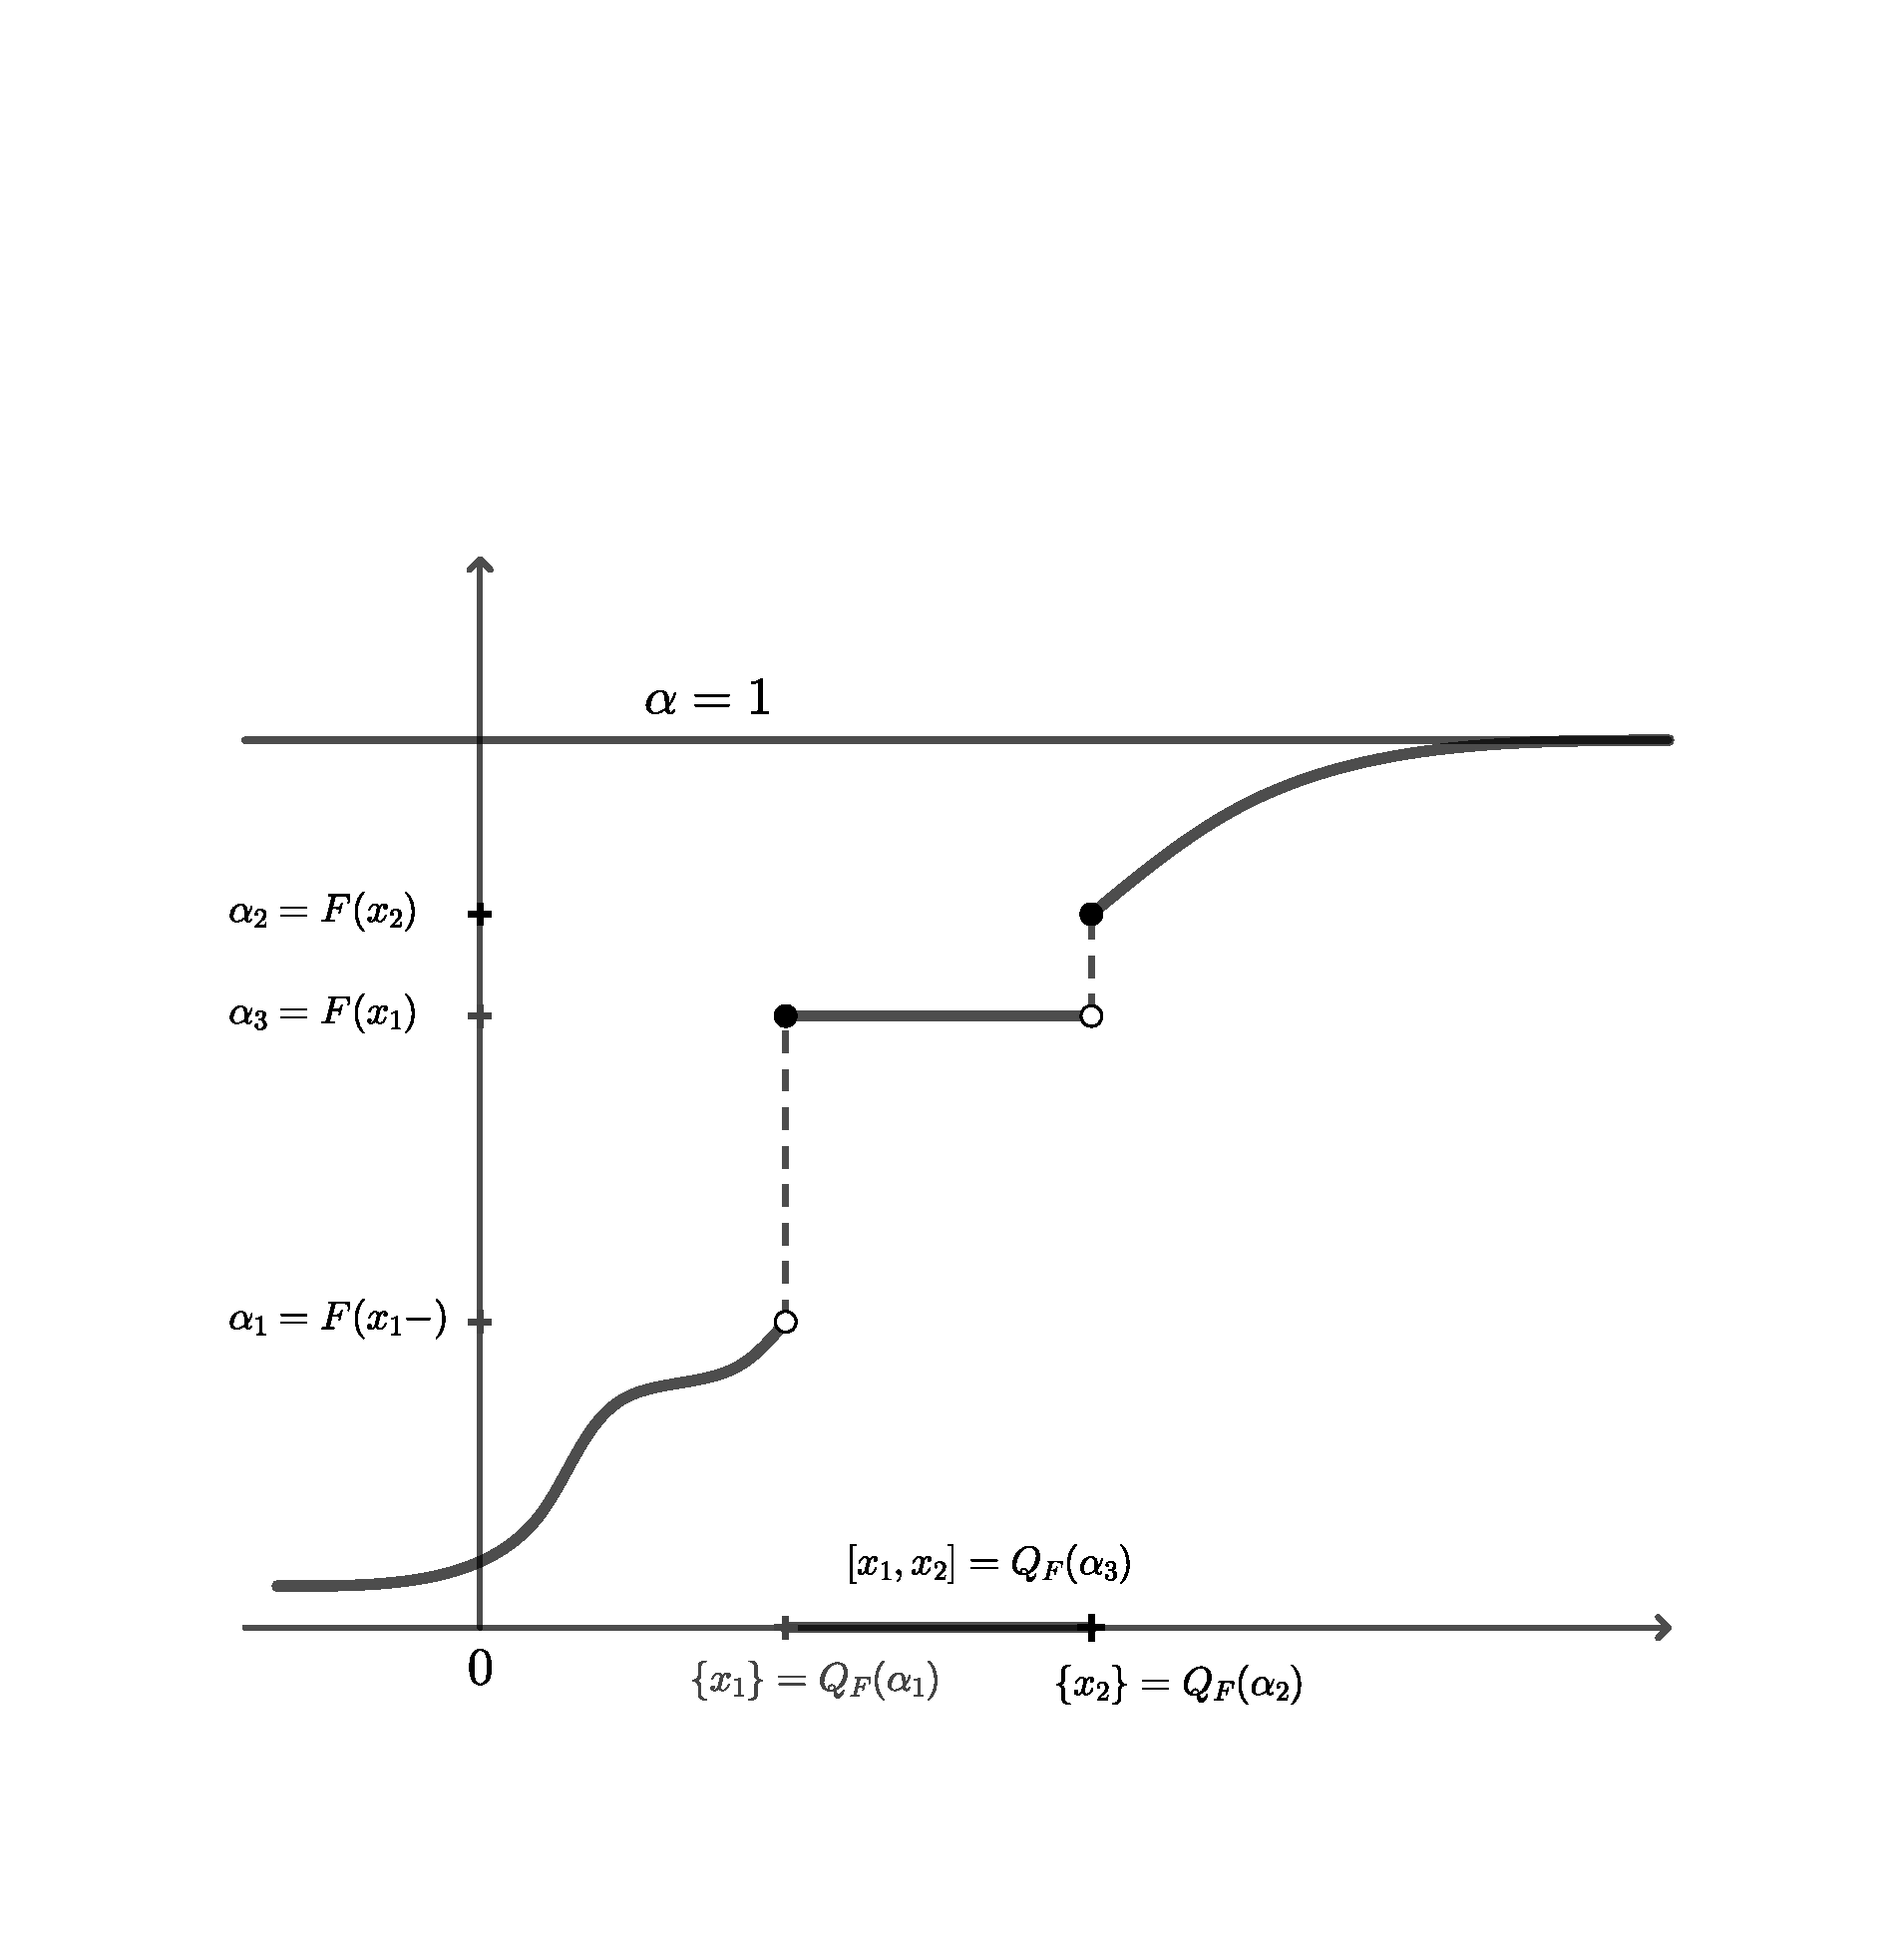
\includegraphics[width=\textwidth]{../figures/FQ.pdf}
\vspace{-15mm}
\caption{Example of a cdf $F$ (with graph including solid line and filled points) superimposed on its 
quantile function $Q_F$ (with graph including dashed and solid lines as well as both filled and empty points).
The notation $F(A)$ should be read as $F(x)$ for any $x\in A$.}
\label{fig:FQ}
\end{figure}

\subsection{Opportunity relative to an oracle}
Quantiles equivalently arise when the decision problem is defined in terms of the random \emph{opportunity} loss 
\begin{align}
l_o(x,Y) := l(x,Y) - l(Y,Y) = Cx + L(Y-x)_{+} - CY \label{eqn:opp-loss}
\end{align}
which expresses how much more loss is realized by the decision $x$ than an oracle would have incurred, knowing to invest exactly
the future value of $Y$. The optimal decision for $\Ex_F[l_o(x,Y)]$ is the same as for $\Ex_F[l(x,Y)]$ since the term $-C\Ex_F[Y]$ is 
constant in $x$, leading again to the inequalities \eqref{eqn:expQd-ineq}.

Opportunity loss \eqref{eqn:opp-loss} rearranges to 
\begin{align}
l_o(x,Y) &= C(x - Y)_{+} + (L-C)(Y-x)_{+} \\
&= L(1-\alpha)(x - Y)_{+} + L\alpha(Y-x)_{+} \\
&= L(\alpha - \mathbf{1}\{Y < x\})(Y-x) \\
&= L \max \left\{(\alpha-1)(Y-x), \alpha(Y-x)\right\}
\end{align}
a form in which it is often called \emph{pinball} loss, despite its graph being an unlikely pinball trajectory for $\alpha \neq 1/2$.


\section{Allocation Bayes acts as vectors of marginal quantiles.}
\label{sec:bayes-quantiles}

Here we show that the Bayes act $x^{F,K} = (x_1^{F,K},\ldots,x_N^{F,K})$ for a forecast $F$, corresponding to the
allocation problem \eqref{eqn:loss_fn} (in Section \ref{sec:methods.detailed.specific_allocation} in the main text) can
be represented as a vector of quantiles for the marginal forecast distributions $F_i$ at a single probability level
$\tau^{F,K}$, that is, $x_i^{F,K} = q_{F_i,\tau^{F,K}}$. An immediate consequence used in the examples in Section \ref
{sec:methods.overview} in the main text is that if $F_i = \mathrm{Exp}(1/\sigma_i)$ for all $i$, then the Bayes act is
proportional to $(\sigma_1,\ldots,\sigma_N)$, since $q_{\mathrm{Exp}(1/\sigma),\tau} = -\sigma \log(1-\tau)$.

For an arbitrary allocation vector $x \in \mathbb{R}^N_{+}$ the expected loss
\begin{align}
\mathbb{E}_{F} [s_A(x, Y)] = \sum_{i=1}^{N} L \cdot \mathbb{E}_{F_i}[(Y_i - x_i)_{+}] \label{eqn:AS_formula}
\end{align} 
is the sum of expected shortages (scaled by $L$) under the allocations $x_i$ in each location. We therefore
have the following necessary condition for $x^{\star} \in \mathbb{R}^N_{+}$ to be an optimal allocation for $\mathbb
{E}_{F} [s_A(x, Y)]$ under the constraint $\sum_{i=1}^{N} x_i = K$: if $\delta > 0$ of the $x_i^{\star}$ units of resource
allocated to location $i$ are reallocated to location $j$, expected shortage will increase in location
$i$ by at least as much as it decreases in location $j$. That is,
\begin{align}
\mathbb{E}_{F_i}[(Y_i - (x^{\star}_i - \delta))_{+}] - \mathbb{E}_{F_i}[(Y_i - x^{\star}_i)_{+}] \geq 
\mathbb{E}_{F_j}[(Y_j - x^{\star}_j)_{+}] - \mathbb{E}_{F_j}[(Y_j - (x^{\star}_j + \delta))_{+}]. \label{eqn:ASoptimal1}
\end{align}
Since the expected shortages in $i$ and $j$ have right and left derivatives at any $x_i$ and $x_j$ (see Section \ref{sec:shortage}), we can
divide \eqref{eqn:ASoptimal1} by $\delta$ and take limits for $\delta \searrow 0$ to get
\begin{align}
-D_{-} \mathbb{E}_{F} [(Y_i - x^{\star}_i)_{+}] \geq -D_{+}\mathbb{E}_{F} [(Y_j - x^{\star}_j)_{+}]. \label{eqn:RLineq}
\end{align}
Note that the minus signs appear because our optimality condition addresses how a \emph{decrease} in resources will \emph{increase}
the expected shortage in $i$ and vice versa in $j$.
Scaling by $L$ to match the right and left partial derivatives of $\mathbb{E}_{F} [s_A(x, Y)]$ and using formulae \eqref{eqn:dsfl} and \eqref{eqn:dsfr}, \eqref{eqn:RLineq} becomes
\begin{align}
L(1-F_i(x^{\star}_i-)) \geq L(1-F_j(x^{\star}_j)). \label{eqn:RLineq2}
\end{align}
Inequalities \eqref{eqn:RLineq} and \eqref{eqn:RLineq2} remain true with $i$ and $j$ reversed. They hold with $i=j$ as well by the
definition of $F_i(x^{\star}_i-)$. Therefore, a number $\lambda$ (a \emph{Lagrange multiplier}) exists, which is independent of $i$,
such that
\begin{align}
L(1-F_i(x^{\star}_i-)) \geq \lambda \geq L(1-F_i(x^{\star}_i)), \quad \text{for all } i \in 1,\ldots,N.
\end{align}
That is,
\begin{align}
F_i(x^{\star}_i) \geq 1 - \lambda/L \geq F_i(x^{\star}_i-),
\end{align}
which says (c.f. discussion after \eqref{eqn:F-alpha-ineq} and \eqref{eqn:set-alpha-ineq}) that $x^{\star}_i$ is a quantile $q_{\tau,F_i}$ for
$\tau = 1 - \lambda/L$.

The constraint now determines $\tau$ (and hence the Bayes act) through 
\begin{align}
\sum_{i=1}^{N} q_{\tau,F_i} = K. \label{eqn:quantiles-sum-to-K}
\end{align}
This equation implies that 
\begin{align}
K \in TQ_F(\tau) \label{eqn:tau-inclusion}
\end{align}
where the set-valued function
\begin{align}
TQ_F(\tau) := \sum_{i=1}^{N} Q_{F_i}(\tau) = \left[\sum_{i=1}^{N} q^{-}_{\tau,F_i}, \sum_{i=1}^{N} q^{+}_{\tau,F_i}\right]
\end{align}
is defined using interval addition $[a,b] + [c,d] = [a+c, b+d]$. (Note that the letter $T$ is being used to connote a ``totalling'' 
operation, as it often is in survey sampling literature.) Conversely, if $\tau^{\star}$ satisfies \eqref{eqn:tau-inclusion}, then
we can find a solution $\bm{q}_{\tau^{\star},F} := (q_{\tau^{\star},F_1},\ldots,q_{\tau^{\star},F_N})$ to 
\eqref{eqn:quantiles-sum-to-K} within the set 
$\undertilde{\bm{F}}^{-1}(\tau^{\star}) \subset \mathbb{R}_{+}^N$ where $\undertilde{\bm{F}}^{-1}(\tau)$  is the 
Cartesian product $(F_1^{-1}(\tau),\ldots,F_N^{-1}(\tau))$.

$TQ_F$ satisfies the conditions mentioned in section \ref{sec:quantile-functions} for being a quantile function, and so there
is a random variable $TY_F$ with cdf $F_{T} := F_{TQ_F}$.  From this perspective, the problem of finding $\tau$ becomes the calculation 
of $F_{T}(K) = \mathbb{P}(TY_F \leq K)$, making clear the existence of a solution $\tau^{\star}$ to \eqref{eqn:tau-inclusion}. This also
yields the interesting formal equation for the Bayes act
\begin{align}
\undertilde{\bm{F}}(x^{F,K}) = \mathbf{1}_N F_{T}(K),
\end{align}
where $\mathbf{1}_N: \mathbb{R} \to \mathbb{R}^N$ is the linear map that takes $a$ to the $N$-vector $(a,\ldots,a)^T$ and the vector of marginal 
cdfs $\undertilde{\bm{F}} := (F_1,\ldots,F_N)$ is a map from $\mathbb{R}^N$ to $\mathbb{R}^N$. 
With this notation we can write \eqref{eqn:tau-inclusion} as
\begin{align}
K \in TQ_F\left(\frac{1}{N} \mathbf{1}^T \undertilde{\bm{F}}(x^{F,K})\right),
\end{align}
which leads conceptually to the iterative numerical method of solving for $\tau$ and $x^{F,K}$ discussed next in section \ref{sec:numeric}. 

Two awkward features of the quantile representation of the Bayes act can arise.  First, point masses in the $F_i$ create point masses for $F_T$ which may cause $\tau^{\star}$ to not be the unique solution to \eqref{eqn:tau-inclusion}. Secondly, if more than 
one $Q_{F_i}(\tau^{\star})$ is a positive-width interval, then the Bayes act will not be unique in these coordinates, and generically
not all points in the $Q_{F_i}(\tau^{\star})$ will be the coordinate of a Bayes act.

It is important to note that $\lambda$ depends on the forecast $F$ and the constraint level $K$. Thus while $\lambda = L(1-\tau)$ can be
interpreted as a kind of ``cost'' imposed by the constraint in the allocation problem which is analogous to $C = L(1-\alpha)$ in the  
the cost-lost problem of section \ref{sec:quantiles_shortage}, it does not serve to define the allocation loss function in the way that $C$ defines \eqref{eqn:expQloss}. $\lambda$ is rather a parameter that must be found, given the pair $F$ and $K$.

\section{Numerical computation of allocation Bayes acts}
\label{sec:numeric}

In practice, \eqref{eqn:quantiles-sum-to-K} is rarely amenable to closed form solution.
Using the Bayes act in explicit computations therefore requires a method of generating an approximation $\tilde{\tau}$ to 
a solution $\tau^{\star}$ of \eqref{eqn:tau-inclusion}.  One would also strive to have some control over a robust measure of 
of the approximation error of the random shortages which we aim to compute using the Bayes act. One possible measure is the sum
of absolute coordinate errors
\begin{align}
\mathrm{SAE}(Y,\tilde{\tau}) = \sum_{i=1}^{N} \left| (Y_i-q_{\tilde{\tau},F_i})_+ - (Y_i-x_i^{F,K})_+ \right|
\end{align}
% of the Bayes risk error or ``optimality gap''
% \begin{align}
% \left|\mathbb{E}_F\left[s_A(\bm{q}_{\tilde{\tau},F}, Y)\right] - \mathbb{E}_F[s_A(x^{F,K}, Y)]\right| = 
% L\left| \sum_{i=1}^{N}\mathbb{E}_{F_i}\left[(Y_i-q_{\tilde{\tau},F_i})_+ - (Y_i-x_i^{F,K})_+\right]\right|
% \end{align}
where $\bm{q}_{\tilde{\tau},F}$ solves the linear program
$\sum_{x \in \undertilde{\bm{F}}^{-1}(\tilde{\tau})}x_i = K$ approximating the true Bayes act defining linear program
$\sum_{x \in \undertilde{\bm{F}}^{-1}(\tau^{\star})}x_i = K$. In this section we outline such a method we have implemented 
in the \verb`R` package \verb`alloscore`.

Suppose we have established that $\tau^{\star} = F_T(K)$ lies in the interval $I_1 = [\tau_L, \tau_U]$ with $\tau_L < \tau_U$,
that is, $K \in [q^{-}_{F_T,\tau_L}, q^{+}_{F_T,\tau_U}]$.
From section \ref{sec:quantile-functions}, we know that the set 
$TQ_F(\tau_L) \cup TQ_F(\tau_U) \subset [q^{-}_{F_T,\tau_L}, q^{+}_{F_T,\tau_U}]$
is arranged in exactly one of the following ways (where e.g. refers to figure \ref{fig:FQ}): 
\begin{itemize}
\item[($\bullet \bullet$)] $TQ_F(\tau_L) \cap TQ_F(\tau_U) = \varnothing$ 
(and $q^{+}_{F_T,\tau_L} < q^{-}_{F_T,\tau_U}$, e.g., $\tau_L=\alpha_1, \tau_U=\alpha_5$)
\item[($\bullet$)] $TQ_F(\tau_L) = \{K\} = TQ_F(\tau_U)$ 
(a point mass at $K$, e.g., $\alpha_3 \leq \tau_L \leq \tau_U \leq \alpha_5$)
\item[($\bullet\!-$)] $TQ_F(\tau_L) = \{q^{-}_{F_T,\tau_U}\} \subsetneq TQ_F(\tau_U)$ 
(a point mass at $q^{-}_{F_T,\tau_U}$, e.g., $\tau_L = \alpha_3, \tau_U = \alpha_5$)
\item[($-\!\bullet$)] $TQ_F(\tau_L) \supsetneq \{q^{+}_{F_T,\tau_L}\} = TQ_F(\tau_U)$ 
(a point mass at $q^{+}_{F_T,\tau_U}$, e.g., e.g., $\tau_L = \alpha_5, \tau_U = \alpha_4$).
\end{itemize}
 
In the case ($\bullet$), we can immediately take 
$\tau^{\star}=\tau_U$ as the probability level representing the allocation Bayes act.
In the cases
($\bullet\!-$), and ($-\!\bullet$), which imply the presence of a point mass in one or more of the 
component forecasts adjacent to a region of zero density in all components, we can take $\tau^{\star}=\tau_U$ or $\tau_L$, 
respectively, as the representing probability level.  
Having found our $\tau^{\star}$ we then arrive at a Bayes act $x^{F,K}$ by by solving the
linear program $\sum_{x \in \undertilde{\bm{F}}^{-1}(\tau^{\star})}x_i = K$.

In the remaining and typical case of ($\bullet \bullet$), further search is generally necessary. We can proceed 
by evaluating $TQ_F$ at $\tau_M = \frac{1}{2}\left(\tau_L + \tau_U\right)$ and replacing $I_1$ with one of its 
halves
\begin{align}
I_2 = 
\begin{cases}
[\tau_L, \tau_M] & \text{ if } K < q^{-}_{F_T,\tau_M} \\
[\tau_M, \tau_U] & \text{ if } K \geq q^{-}_{F_T,\tau_M}
\end{cases}
\end{align}
which also contains $\tau^{\star} = F_T(K)$. This follows from the definition $q^{-}_{F_T,\tau_M} := \min\{x \mid F_T(x) \geq \tau_M\}$, 
according to which
\begin{align}
\begin{cases}
K < q^{-}_{F_T,\tau_M} \text{ implies } \tau^{\star} = F_T(K) < \tau_M  \\
K \geq q^{-}_{F_T,\tau_M} \text{ implies } \tau^{\star} = F_T(K) \geq \tau_M.
\end{cases}
\end{align}
Note that $K \leq q^{-}_{F_T,\tau_M}$ would not imply $F_T(K) \leq \tau_M$ due to the possibility of a point mass at $K$.

Iterating this process we obtain a sequence $\{I_k\}, k=1,2,\ldots$ of intervals of widths 
$\left|I_k \right| = 2^{1-k}\left|I_1 \right|$ which either terminates at one of the scenarios 
($\bullet$), ($\bullet\!-$), or ($-\!\bullet$), or provides infinite sequences $\{\tau_{L,k}\}$ and $\{\tau_{U,k}\}$ converging
to $\tau^{\star}$ from below and above. Such a sequence provides the basis of a ``bisection'' algorithm for finding
the ``root'' $\tau^{\star}$ of the set condition $0 \in TQ_F(\tau) - K$.

In the generic case of an infinite $\{I_k\}$, we need to define practical stopping criteria for the possible limit behaviours of 
$F_T(K \pm \varepsilon)$ as $\varepsilon \searrow 0$ which are exemplified in figure \ref{fig:FQ} at $0, x_1, x_2, x_3, (x_3 +x_4)/2$ and 
$x_5$.
% \begin{itemize}
% \item[($\mathrlap{\,\bullet}{\,/}\,$)] $F_T(K - \varepsilon) < F_T(K-) = F_T(K) < F_T(K + \varepsilon)$
% (so that $\tau^{\star} = F_T(K-)$ and $TQ_F(\tau^{\star}) = \{K\}$)
% \item[($/\!\!\raisebox{.9ex}{$\bullet$\!-}$)] $F_T(K - \varepsilon) < F_T(K-) = F_T(K) = F_T(K + \varepsilon)$
% \item[($\raisebox{-.9ex}{-\!$\bullet$}\!\!/$)] $F_T(K - \varepsilon) = F_T(K) < F_T(K + \varepsilon)$
% \item[($\raisebox{-.9ex}{\phantom{-}\!$\bullet$}\!\!/$)] $F_T(K - \varepsilon) \leq F_T(K-) < F_T(K) < F_T(K + \varepsilon)$
% \item[($\,\bullet\!\text{-}$)] $F_T(K - \varepsilon) \leq F_T(K-) < F_T(K) = F_T(K + \varepsilon)$
% \item[($\text{-}\!\!\bullet\!\!\text{-}$)]  $F_T(K - \varepsilon) = F_T(K) = F_T(K + \varepsilon)$
% so that $K \in (q^{-}_{F_T,\tau^{\star}}, q^{+}_{F_T,\tau^{\star}})$ and all component forecasts $F_i$ have 
% zero density at points $x_i \in (q^{-}_{F_i,\tau^{\star}}, q^{+}_{F_i,\tau^{\star}})$ and $\sum x_i = K$.
% \end{itemize}

And after having obtained sufficiently a sufficient narrow terminal $I_K = [\tau_{L,K}, \tau_{U,K}]$ we need a protocol for 
how to select a solution to the linear program $\sum_{x \in \undertilde{\bm{F}}^{-1}(I_K)}x_i = K$ as an approximate Bayes act.

\section{Computing allocations from finite quantile forecast representations}

In section 3 of the manuscript, we used the allocation score to evaluate forecasts of COVID-19 hospitalizations that have been submitted to the COVID-19 Forecast Hub. These forecasts are submitted to the Hub using a set of 23 quantiles of the forecast distribution at the 23 probability levels in the set $\mathcal{T} = \{0.01, 0.025, 0.05, 0.1, 0.15, \ldots, \allowbreak 0.9, 0.95, 0.975, 0.99\}$, which specify a predictive median and the endpoints of central $(1 - \alpha) \times 100\%$ prediction intervals at levels $\alpha = 0.02, 0.05, 0.1, 0.2, \allowbreak 0.3, 0.4, 0.5, 0.6, \allowbreak 0.7, 0.8, 0.9$. For a given week and target date, we use $q_{i,k}$ to denote the submitted quantiles for location $i$ and probability level $\tau_k \in \mathcal{T}$, $k = 1, \ldots, 23$.

In the event that there is some $k \in \{1, \ldots, 23\}$ for which $\sum_i q_{i,k} = K$, i.e., the provided predictive quantiles at level $\tau_k$ sum across locations to the resource constraint $K$, the solution to the allocation problem is given by those quantiles. However, generally this will not be the case; the optimal allocation will typically be at some probability level $\tau^\star \notin \mathcal{T}$.

To address this situation and support the numerical allocation algorithm outlined in section \ref{sec:numeric}, we need a mechanism to approximate the full cumulative distribution functions $F_i$, $i = 1, \ldots, N$ based on the provided quantiles. We have developed functionality for this purpose in the \verb`distfromq` package for R (cite). This functionality represents a distribution as a mixture of discrete and continuous parts, and it works in two steps:
\begin{enumerate}
  \item Identify a discrete component of the distribution consisting of zero or more point masses, and create an adjusted set of predictive quantiles for the continuous part of the distribution by subtracting the point mass probabilities and rescaling.
  \item For the continuous part of the distribution, different approaches are used on the interior and exterior of the provided quantiles:
  \begin{enumerate}
    \item On the interior, a monotonic cubic spline interpolates the adjusted quantiles representing the continuous part of the distribution.
    \item A location-scale parametric family is used to extrapolate beyond the provided quantiles. The location and scale parameters are estimated separately for the lower and upper tails so as to obtain a tail distribution that matches the two most extreme quantiles in each tail.
  \end{enumerate}
\end{enumerate}
The resulting distributional estimate exactly matches all of the predictive quantiles provided by the forecaster. We use the cumulative distribution function resulting from this procedure as an input to the allocation score algorithm.

We refer the reader to the \verb`distfromq` documentation for further detail.

% \begin{enumerate}
%   \item First, we handle settings where the provided quantiles imply the existence of one or more point masses. Specifically, if there are distinct probability levels $\tau_k < \tau_{k^\prime}$ that have the same quantiles, $q_{l,k} = q_{l, k^\prime}$, the distribution contains a point mass at $q_{l,k}$. We split into three cases depending on the number of distinct provided quantiles:
%   \begin{enumerate}
%     \item If all provided quantiles are equal to each other, we infer that the distribution consists of a single point mass at that quantile value.
%     \item If there are two distinct quantiles across all of the probability levels $\tau_k \in \mathcal{T}$, our estimated distribution consists of a mixture of two point masses. The probability assigned to the point mass at $q$ is proportional to $\tau_q^\max - \tau_q^\min$, where
%     $$\tau_q^\max = \begin{cases}
%       \max_{\{\}} \tau_k
%     \end{cases}$$ is the largest probability level $\tau_k$ for which $q_{l,k} = q$, and $\tau_q^\min$ is defined similarly.
%     \item Otherwise, our final estimate will consist of a mixture of a discrete distribution with point masses at the duplicated quantiles and a continuous distribution elsewhere. In this step, we  In this case, the discrete distribution has point mass probabilities calculated as $d_q = \tau_q^\max - \tau_q^\min$, where $\tau_q^\max$ and $\tau_q^\min$ are defined as in the previous point.
%   \end{enumerate}
% \end{enumerate}

\section{Propriety of the allocation score}
\label{sec:proper}

In order for a scoring rule to be guaranteed to yield logically consistent forecast evaluations, it must be \emph{proper}, which means,
in essence, that a forecaster cannot perceive any forecast that is at odds with their beliefs about the events being forecasted as having an optimal expected score.
We formalize this in terms of forecaster ``self-assessment'' in section \ref{sec:proper_def} and then address the propriety of the allocation score in two stages:
\begin{itemize}
  \item Section \ref{sec:alloscore_proper} shows that the allocation score is proper when the forecaster's actual forecast distribution $F$ is available (as is any score derived using the decision theoretic procedures outlined in section 2 of the manuscript)
  \item Section \ref{sec:distfromq_alloscore_proper_prospective} addresses the propriety of an analysis that combines an approximate parametric representation of the forecast distribution and evaluation with the allocation score. It shows that this procedure yields a proper score so long as this representation and scoring procedure was specified prospectively by the hub. This includes the use of methods such as \verb`distfromq` for constructing forecast distributions as a special case. However,  \emph{post hoc} application of this scoring procedure to quantile forecasts is improper.
\end{itemize}

\subsection{Proper scores}
\label{sec:proper_def}

Expanding on the decision theoretic perspective sketched in Section \ref{sec:quantiles_shortage}, we can view a loss function 
as a general tool for formalizing a decision problem that assigns numerical value to the \emph{result} of taking an \emph{action} $x$
in preparation for an \emph{outcome} $y$. Here, we consider a setting where the individual making the decision is the forecaster, and the action is to report a particular forecast.

A \emph{scoring rule} $S$ is a loss function where the action 
is a probabilistic forecast $F$ of the outcome $y$ (or the statement of $F$ by a forecaster). Just as in 
Section \ref{sec:quantiles_shortage}, given an action $F$, $S$ transforms a random outcome variable $Y$ into a random loss $S(F,Y)$. 
We refer to the realized loss $S(F,y)$ as the \emph{score} of $F$ at $y$.

Decision theoretically, probabilistic forecasts are a unique kind of action in that they can be used to generate their
own (simulated) outcome data, against which they can be scored using $S$. $S$ therefore commits a probabilistic forecast
$F$ to the ``self-assessment'' $\Ex [S(F, Y^F)]$, where $Y^F \sim F$ is the random variable defined by sampling from
$F$, as well to an assessment $\Ex [S(G, Y^F)]$ of any alternative forecast $G$.

A natural consistency criterion for $S$ is that it does not commit $F$ to assessing any other forecast $G$ as being better than $F$ itself, that is, that
\begin{align}
\Ex [S(F, Y^F)] \leq \Ex [S(G, Y^F)] \label{eqn:prop_ineq}
\end{align} 
for any $F,G$. Otherwise, the optimal decision for some forecaster would be to state a forecast $G$ other than the forecast $F$
which they believe describes the outcome $Y$.
A scoring rule meeting this criterion is called \emph{proper}.  The inequality can also be written 
as $\Ex_F [S(F, Y)] \leq \Ex_F [S(G, Y)]$ where the subscript specifies the distribution of $Y$.  
$S$ is \emph{strictly proper} when this inequality is sharp, in which case the \emph{only} optimal decision for a forecaster is to state
the forecast they believe to be true.

\subsection{The allocation score is proper}
\label{sec:alloscore_proper}

We recall the three-step decision theoretic procedure for deriving proper scoring rules that we outlined in section \ref{sec:methods.detailed.decisiontheory} of the main text:
\begin{enumerate}
  \item Specify a \emph{loss function} $s(x, y)$ that measures the loss associated with taking action $x$ when outcome $y$ eventually occurs.
  \item Given a probabilistic forecast $F$, determine the \emph{Bayes act} $x^F$ that minimizes the expected loss under the distribution $F$.
  \item Define a \emph{scoring rule} which assigns the loss realized by the Bayes act $x^F$ against outcome $y$ as the score of $F$ at $y$:
  \begin{align}
    S(F, y) = s(x^F, y). \label{eqn:bayes_sr}
  \end{align}
\end{enumerate}

Such scoring rules, which we call \emph{Bayes scoring rules}, are proper by construction since
\begin{align}
\Ex_F [S(F, Y)] &= \Ex_F [ s(x^F, Y) ] \nonumber \\
 &= \min_{x} \Ex_F [ s(x, Y) ] \quad \text{ (by definition of $x^F$)} \\
 &\leq \Ex_F [ s(x^G, Y) ] \label{eqn:dt_proper_key} \\
 &= \Ex_F [ S(G, Y)]. \nonumber
\end{align}

The allocation scoring rule is Bayes and therefore proper.

We note that in the probabilistic forecasting literature (see e.g., \cite{gneiting2011making}, Theorem 3) what we have 
termed Bayes scoring rules typically appear via \eqref{eqn:bayes_sr} where $x^F$ is some given functional of $F$ which 
can be shown to be \emph{elicitable}, that is, to be the Bayes act for some loss function $s$.
Such a loss function is said to be a \emph{consistent loss (or scoring) function} for the functional $F \mapsto x^F$, and many important
recent results in the literature (e.g., \cite{fisslerziegel2016consistency}) address whether there \emph{exists} any loss 
function for $x^F$ which is consistent. Our orientation
is different from this insofar as we \emph{begin} by specifying a decision problem and a loss function of subject matter relevance
and use the Bayes act only as a bridge to a proper scoring rule.  Consistency is never in doubt.

\subsection{Prospectively-specified use of the allocation score to evaluate forecasts approximately represented as members of a parametric family is proper}
\label{sec:distfromq_alloscore_proper_prospective}

In practice, open forecasting exercises are generally not able to collect an exact representation of the forecast distribution $F$ other than in simple settings such as for a categorical variable with a relatively small number of categories. In settings where the outcome being forecasted is a continuous quantity (such as rates of influenza-like illness among outpatient doctor visits) or a count (such as influenza hospitalizations), forecasting exercises have therefore resorted to collecting summaries of a forecast distribution such as bin probabilities or predictive quantiles. This raises the question of whether use of the allocation score still consitutes a proper evaluation procedure if the forecast distribution $F$ is not itself directly recorded. The answer we provide in this section is that it is, so long as the fact that the allocation score will be used for forecast evaluation and the method that will be used to obtain a distributional estimate of $F$ from the provided forecast representation are communicated to participating forecasters prospectively.

We consider a setting where a forecasting exercise (such as a forecast hub) pre-specifies that forecasts will be represented using a parametric family of forecast distributions $G_\theta(y)$, and the task of the forecaster is to select a particular parameter value $\theta$. We use $\mathcal{P}$ to denote the collection of all distributions $G_\theta$ in the given parametric family. For instance, it has recently been proposed that mixture distributions could be used to represent forecast distributions \cite{wadsworth2023mixture}. Additionally, we note that the functionality in \verb`distfromq` can be viewed as specifying a parametric family $\mathcal{P}_{\mathrm{dfq}}$ where the parameters $\theta$ of $G_\theta$
are its quantiles at pre-specified probability levels, and where the shape of any $G_\theta \in \mathcal{P}_{\mathrm{dfq}}$ over the full range of its support is entirely controlled by these quantiles.

We find it helpful now to formally distinguish between two decision making problems. The first is the public health decision maker's allocation problem where the task is to select an allocation $x$, with the allocation loss $s_A(x, y) = \sum_{i=1}^N L \cdot \max(0, y_i - x_i)$ as described in section \ref{sec:methods.detailed.specific_allocation} of the main text.
The second is the forecaster's reporting problem where the task is to select parameter values $\theta$ to report. The forecaster's loss is given by $s_R(\theta, y) = s_A(x^{G_\theta}, y)$, where $x^{G_\theta}$ is the Bayes act for the allocation problem under the distribution $G_\theta$. In words, the loss associated with reporting $\theta$ is equal to the loss associated with taking the Bayes allocation corresponding to the distribution $G_\theta$.

Following our usual construction, the Bayes act for the forecast reporting problem is the parameter set that minimizes the forecaster's expected loss. Breaking with our earlier notation for improved legibility, we use $\theta^\star(F)$ to denote this Bayes act:
\begin{align*}
\theta^\star(F) &= \text{argmin}_\theta \Ex_F [s_R(\theta, Y)] \\
&= \text{argmin}_\theta \Ex_F [s_A(x^{G_\theta}, Y)]
\end{align*}

We then arrive at the scoring rule
$$S_R(F, y) = s_R(\theta^\star(F), y) = s_A(x^{G_{\theta^\star(F)}}, y).$$
It follows from the discussion in section \ref{sec:alloscore_proper} that this is a proper scoring rule for $F$. Additionally, we note that the score can be calculated from the reported parameter values $\theta^\star(F)$.

We emphasize that the forecaster's true predictive distribution $F$ does not need to be a member of the specified parametric family $\mathcal{P}$ for this construction to yield a proper score.
It is, however, necessary to specify the parametric family to use and the foundational scoring rule $s_A$ (including any relevant problem parameters such as the resource constraint $K$) in advance, so that forecasters can identify the Bayes act parameter set $\theta^\star(F)$ to report.

If the parametric family used to represent forecast distributions is flexible enough, the reporting scoring rule $S_R$ and the allocation score are equivalent in the sense that they will yield the same score for any distribution $F$.
Suppose that for a given resource constraint $K$, for any forecast distribution $F$ it is possible to find a member $G_{\theta^\star}$ of the specified parametric family $\mathcal{P}$ with the same allocation as $F$ (i.e., $x^F = x^{G_{\theta^\star}}$). Then $\theta^\star$ is a Bayes act for the reporting problem since for any other parameter value $\theta$,
\begin{align*}
\Ex_F[s_R(\theta^\star, Y)] &= \Ex_F[ s_A(x^{G_{\theta^\star}}, Y) ] \\
&= \Ex_F[s_A(x^F, Y)]  \quad \text{ (since $x^F = x^{G_{\theta^\star}}$)} \\
&\leq \Ex_F[ s_A(x^{G_\theta}, Y) ]  \quad \text{ (by definition of $x^F$)} \\
&= \Ex_F[ s_R(\theta, Y)].
\end{align*}
It therefore follows that
\begin{align*}
S_R(F, y) &= s_R(\theta^\star, y) \\
&= s_A(x^{G_{\theta^\star}}, y) \\
&= s_A(x^F, y) \\
&= S_A(F, y).
\end{align*}

For the particular choice of the parametric family $\mathcal{P}_{\text{dfq}}$ (i.e., using the \verb`distfromq` package), this flexibility requirement is satisfied. For instance, the forecaster could pick one required quantile level (such as 0.5, for which the corresponding predictions are predictive medians), and set the submitted quantiles of their forecast distribution at that level to be the desired allocations.
However, this representation of the forecast may be quite different from the actual forecast distribution $F$.

A key observation is that a \emph{post hoc} analysis combining \verb`distfromq` with the allocation score does not in general yield a proper evaluation method. This is because the forecast distribution $F$ and the distribution $G_\theta \in \mathcal{P}_{\text{dfq}}$ with the same quantiles as $F$ may determine quite different resource allocations, particularly if the tail extrapolations performed by \verb`distfromq` do not match the tail behavior of $F$.

As another alternative for practical forecasting exercises, a forecast hub could ask forecasters to directly provide the Bayes allocations associated with their forecasts for one or more specified resource constraints $K$. At the cost of increasing the number of quantities solicited by the forecast hub, this would have several advantages: it would prevent any artificial distortion of the forecast distributions, allow for direct calculation of scores, and narrow the gap between model outputs and public health end users. For this to be feasible, implementations of the allocation algorithm would have to be provided to participating forecasters in the computational languages being used for modeling.

\bibliography{allocation}

\end{document}
